\documentclass[3p,times]{elsarticle}
\usepackage[utf8]{inputenc}

\usepackage{amssymb,amsmath,latexsym}
\usepackage{soul,color}
\usepackage{xcolor}
\usepackage{graphicx,amssymb,amsmath}
\usepackage{algorithm}
\usepackage[noend]{algpseudocode}
\usepackage{pgfplots}
\usepackage{array}
\usepackage[utf8]{inputenc}
\newcolumntype{P}[1]{>{\centering\arraybackslash}p{#1}}
\usepackage{tikz}
\usepackage{caption}
\setcounter{secnumdepth}{4}
\usepackage{pgfplots}
\usepackage{hyperref}
\usepackage{float}
\usepackage{subcaption}
\pgfplotsset{compat=newest}
\usepackage[utf8]{inputenc}
\usepackage{hyperref}
\usepackage{array}
\usepackage{graphicx}
%\usepackage{authblk}
\usepackage{multirow}

\usepackage[outdir=./]{epstopdf}
\usepackage{dblfloatfix}
\usepackage[figuresright]{rotating}

%\pagecolor[rgb]{0.25,0.25,0.25} %black
%\color[rgb]{0.9,0.9,0.9} %grey

\usepackage{ecrc}

\makeatletter %% <- make @ usable in command sequences
\newcount\SOUL@minus
\makeatother  %% <- revert @

%% The ecrc package defines commands needed for running heads and logos.
%% For running heads, you can set the journal name, the volume, the starting page and the authors

%% set the volume if you know. Otherwise `00'
\volume{00}

%% set the starting page if not 1
\firstpage{1}

\setlength{\textfloatsep}{5pt}
%% Give the name of the journal
\journalname{Computer Speech and Language}

%% Give the author list to appear in the running head
%% Example \runauth{C.V. Radhakrishnan et al.}
\runauth{Anidjar et al.}

%% The choice of journal logo is determined by the \jid and \jnltitlelogo commands.
%% A user-supplied logo with the name <\jid>logo.pdf will be inserted if present.
%% e.g. if \jid{yspmi} the system will look for a file yspmilogo.pdf
%% Otherwise the content of \jnltitlelogo will be set between horizontal lines as a default logo

%% Give the abbreviation of the Journal.
\jid{procs}

%% Give a short journal name for the dummy logo (if needed)
\jnltitlelogo{Speech Recognition}

%% Hereafter the template follows `elsarticle'.
%% For more details see the existing template files elsarticle-template-harv.tex and elsarticle-template-num.tex.

%% Elsevier CRC generally uses a numbered reference style
%% For this, the conventions of elsarticle-template-num.tex should be followed (included below)
%% If using BibTeX, use the style file elsarticle-num.bst

%% End of ecrc-specific commands
%%%%%%%%%%%%%%%%%%%%%%%%%%%%%%%%%%%%%%%%%%%%%%%%%%%%%%%%%%%%%%%%%%%%%%%%%%

\newcommand\MyBox[2]{
  \fbox{\lower0.75cm
    \vbox to 1.7cm{\vfil
      \hbox to 1.7cm{\hfil\parbox{1.4cm}{#1\\#2}\hfil}
      \vfil}%
  }%
}

\begin{document}

\begin{frontmatter}


\title{Vision-Based Automatic Landing of Drones}




\author[a,b,c,d]{Or Haim Anidjar\corref{cor1}}
\ead{orhaim@ariel.ac.il}

\author[a]{Moria Grohar}
\ead{moriagro@gmail.com}

\author[a]{Shirel Turgeman}
\ead{shirel.zz10@gmail.com}

\author[a]{Adi Peisach}
\ead{adi.peisach@gmail.com}

\author[a, b, c]{Boaz Ben-Moshe}
\ead{benmo@ariel.ac.il}


\address[a]{School of Computer Science, Ariel University, Golan Heights 1, 4077625, Ariel, Israel.}

\address[b]{Ariel Cyber Innovation Center, Ariel University, Golan Heights 1, 4077625, Ariel, Israel.}

\address[c]{Kinematics and Computational Geometry Lab (K\&CG), Ariel University, Golan Heights 1, 4077625, Ariel, Israel.}

\address[d]{Data Science and Artificial Intelligence Research Center, Ariel University, Golan Heights 1, 4077625, Ariel, Israel.}

\cortext[cor1]{Corresponding author: Or Haim Anidjar, School of Computer Science, Ariel University, Golan Heights 1, 4077625, Ariel, Israel.}



\begin{abstract}
This article introduces a platform designed to enable precise landings on the edge of rooftops, facilitating operations at boundary locations. The platform integrates voice recognition capabilities for activation, eliminating reliance on manual button controls. The primary objective is to develop a methodology and control algorithm that allows drones to guard settlements effectively. This research employs a combination of straight-line detection and object detection, avoiding the use of global positioning systems. The system is engineered to operate with drones equipped with existing cameras, obviating the need for additional sensors, and is implemented using the DJI SDK on Android devices. This paper presents a visual landing technology through a proposed algorithm, which is divided into two key tasks: scene evaluation and landing site security. Initially, the drone utilizes object detection to identify and avoid obstacles within the landing area, enabling autonomous descent planning. Once obstacles are cleared, the drone transitions to descent mode. For precise landings at the edge of a rooftop, an edge detection algorithm is employed alongside a target line selection process, allowing the user to designate a specific landing line beforehand, ensuring accuracy during the final approach.

\end{abstract}

\begin{keyword}
Visual-Based Landing; Autonomous Landing; Accurate Landing; Spoken Language Recognition.
\end{keyword}

\end{frontmatter}

\section{Introduction}
Unmanned aerial vehicles (UAVs), commonly known as drones, are aircraft that operate without an onboard pilot, controlled either through radio remote systems or autonomous onboard programs. Drones are valued for their simple yet effective design, ease of operation, flexibility, and cost-efficiency, making them versatile tools in both military and civilian domains. In military operations, they play crucial roles in tasks such as tactical reconnaissance, territorial surveillance, and target acquisition. On the civilian side, drones are utilized for activities like environmental monitoring, weather data collection, and infrastructure inspection. As drones become increasingly prevalent in both sectors, ensuring their safe operation—particularly during landing—has emerged as a critical concern.\\Autonomous drone operations have rapidly advanced, yet precision landing remains a significant challenge, especially in environments where GPS signals are unreliable or unavailable. GPS signals can be easily disrupted by various factors: (a) weather conditions and sunspots may weaken signals, although they typically do not hinder positioning; (b) electromagnetic interference from sources like radios and strong magnetic fields can cause varying degrees of disruption; (c) signal strength diminishes under shelters such as buildings, vehicles, insulation materials, trees, and metal components; and (d) high-rise buildings and dense urban areas can severely impact GPS signal quality. Traditional drone landing methods often rely on GPS, which proves inadequate in urban or indoor settings. This limitation poses significant challenges for applications requiring precise landings, such as urban package delivery, infrastructure inspection, and emergency response. As a result, there is a critical need to develop autonomous positioning and flight control systems for drones that do not rely on GPS signals.\\
This research addresses these challenges by developing a visual-based landing system that enhances accuracy and safety. Our approach enables drones to autonomously identify and land on planar surfaces, such as rooftops, relying solely on visual data from the onboard camera. By eliminating the need for additional sensors or external data inputs, this system offers a robust solution for autonomous landings in complex environments.

\subsection{Authors Contribution}
We propose a visual processing framework that enables the drone to autonomously land by utilizing object (obstacle) detection and edge detection. Our approach is tested on a DJI drone equipped with a standard camera, using the DJI SDK for implementation on Android devices. Additionally, we have implemented a "guard" mode in the app—a button that, when activated, is designed to detect movement (such as people, cars, etc.) and send alerts. The system's robustness is further enhanced by incorporating basic voice commands through a speech recognition module, meeting the requirements outlined by MAFAT.

\begin{figure}[htp]
    \centering
    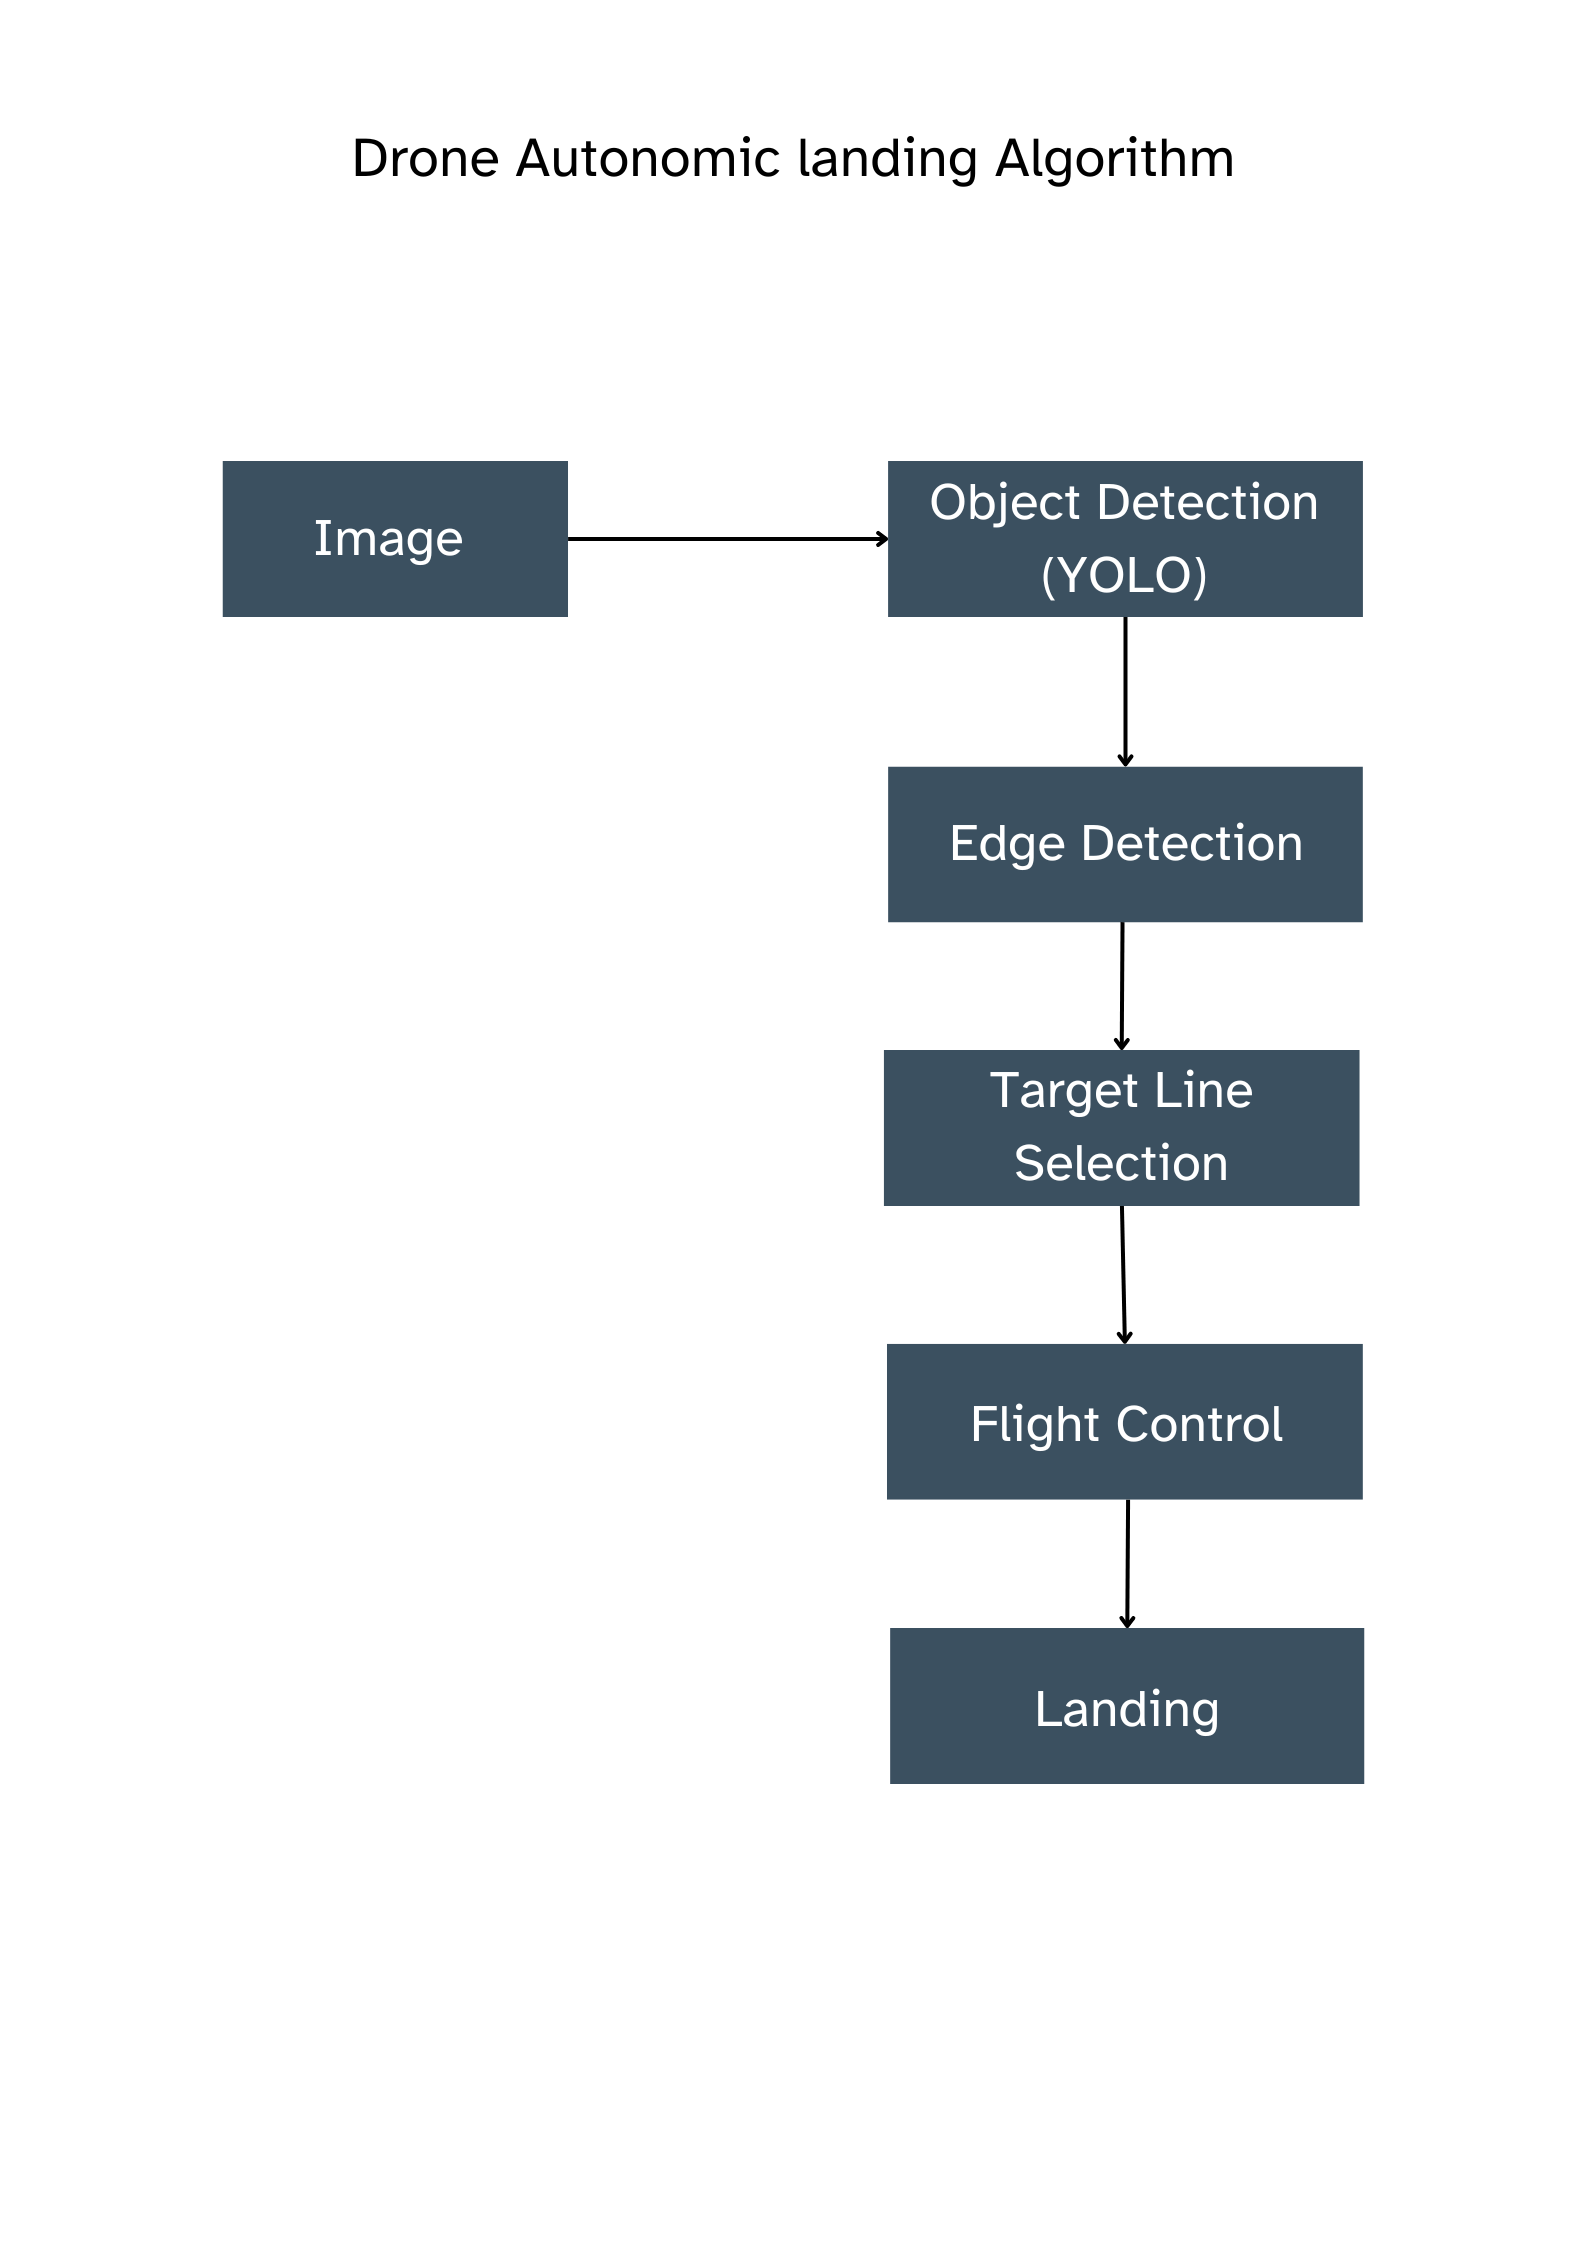
\includegraphics[width=11.0cm]{Schematic_for_automatic_landing.png}
    \caption{Schematic for automatic landing.}
    \label{fig:Schematic_for_automatic_landing.}
\end{figure}


% \subsection{Paper Structure}
% This paper is structured as follows: Section \ref{sec:related} discusses related work in autonomous drone landing and visual navigation. Section \ref{sec:datasets} details the datasets used for testing and validation. Section \ref{sec:framework} describes the proposed framework, including the algorithms and implementation details. Section \ref{sec:exp_eval} presents the experimental evaluation and results. Finally, Section \ref{sec:discussion} offers a discussion on the findings, and Section \ref{sec:conclusions} concludes the paper with suggestions for future work.


% \begin{table}[th]
%   \caption{List of abbreviations}

%   \centering
%   \begin{tabular}{ |c|c|c|}
%   \hline
%     \multicolumn{1}{|c|}{\textbf{Abbreviation}} &
%     \multicolumn{1}{|c|}{\textbf{Meaning}}\\\hline
%     PID & \quad Proportional Integral Derivative \\\hline

%   \end{tabular}
%   \label{tab:list_of_abbreviations}
% \end{table}




\section{Related Work} \label{sec:related}
\subsection{Obstacle Avoidance}
Obstacle avoidance is a critical aspect of autonomous drone operations, especially in dynamic environments where both static and moving obstacles are present. One approach is integrating depth images with an occupancy voxel map to detect and track dynamic obstacles \cite{xu2023real}. This approach effectively balances computational efficiency with the need for accurate detection and tracking, making it suitable for real-time UAV operations. Another approach is.... \cite{redmon2017yolo9000}

% \cite{lee2022camera} is a set.


% Spoken language recognition (SLR) has been a


\section{Datasets} \label{sec:datasets}



In the field of speech recognition, the ability to accurately transcribe




\section{Framework} \label{sec:framework}





\section{Experimental Evaluation and Results} \label{sec:exp_eval}



In accordance with the methodologies outlined in the framework, several modifications were independently evaluated. Below is a tabulated comparison illustrating the differences among these variations, as in Table~\ref{tab:results_comparison}:

\begin{table}[ht]
\centering
\caption{Comparative Analysis of Model Improvements on Validation Dataset.}
\label{tab:results_comparison}
\resizebox{0.4\textwidth}{!}{%
\begin{tabular}{|c|c|}
\hline
\textbf{Model} & \textbf{Accuracy} \\
\hline
Baseline & 0.54 \\

\hline
\end{tabular}%
}
\end{table}


Figure~\ref{fig:conf_matrix_test} depicting the confusion matrices for the final model on :

\begin{figure}[htp]
    \centering
    \includegraphics[width=11.0cm]{con_matrix_test.jpeg}
    \caption{Confusion Matrix on Validation Dataset for the Final Model, showing minimal error.}
    \label{fig:conf_matrix_test}
\end{figure}



The results in Eq.(\ref{eq:inequality}) clearly demonstrate that Boaz has no idea in equations.

\begin{equation} \label{eq:inequality}
    3 \neq 3
\end{equation}


\section{Discussion} \label{sec:discussion}

Advancements in language recognition technologies have been noteworthy, yet they confront several challenges and limitations. This discussion highlights some of the prevalent issues:

\begin{enumerate}

    \item \textbf{Linguistic Ambiguity.} Distinguishing between languages with shared linguistic traits

    \item \textbf{Code-Switching Phenomenon.} In multilingual settings,

\end{enumerate}


\section{Conclusions and Future Work} \label{sec:conclusions}


In this study, we have



% \bibliographystyle{model5-names}\biboptions{authoryear}
% \bibliography{main}
\bibliographystyle{plain}
\bibliography{myDoc}
\end{document}
